\documentclass[aspectratio=169,11pt]{beamer}

\usetheme{Madrid}
\usecolortheme{default}
\usefonttheme{professionalfonts}
\setbeamertemplate{navigation symbols}{}
\setbeamertemplate{footline}[frame number]

\usepackage{amsmath, amssymb, booktabs, graphicx}
\graphicspath{{../../assets/figures/}{assets/figures/}}

\title{Behavioral Frictions and an Introduction to Behavioral Labor}
\subtitle{Labor I -- Week 12}
\author{Teaching deck draft}
\date{}

\begin{document}

\begin{frame}
  \titlepage
\end{frame}

\begin{frame}{Central question and why this is an introduction}
\begin{itemize}
    \item Week 12 is not a list of biases. It is a framework for adapting worker-side labor models when preferences, beliefs, or decision-making depart from the fully rational benchmark.
    \item The key discipline questions are: relative to what benchmark, on which labor margin, with what identifying variation, and with what welfare object?
    \item This is the bridge from Labor I into a full Behavioral Labor course.
\end{itemize}
\end{frame}

\begin{frame}{Why behavioral labor belongs at the end of Labor I}
\begin{itemize}
    \item Week 3: dynamic labor supply gives the benchmark for self-control and continuation values.
    \item Week 7: job amenities gives the benchmark for identity, salience, and job valuation.
    \item Week 11: take-up and delivery design gives the benchmark for complexity, attention, and effective exposure.
\end{itemize}
\end{frame}

\begin{frame}{DellaVigna taxonomy adapted to labor}
\begin{center}
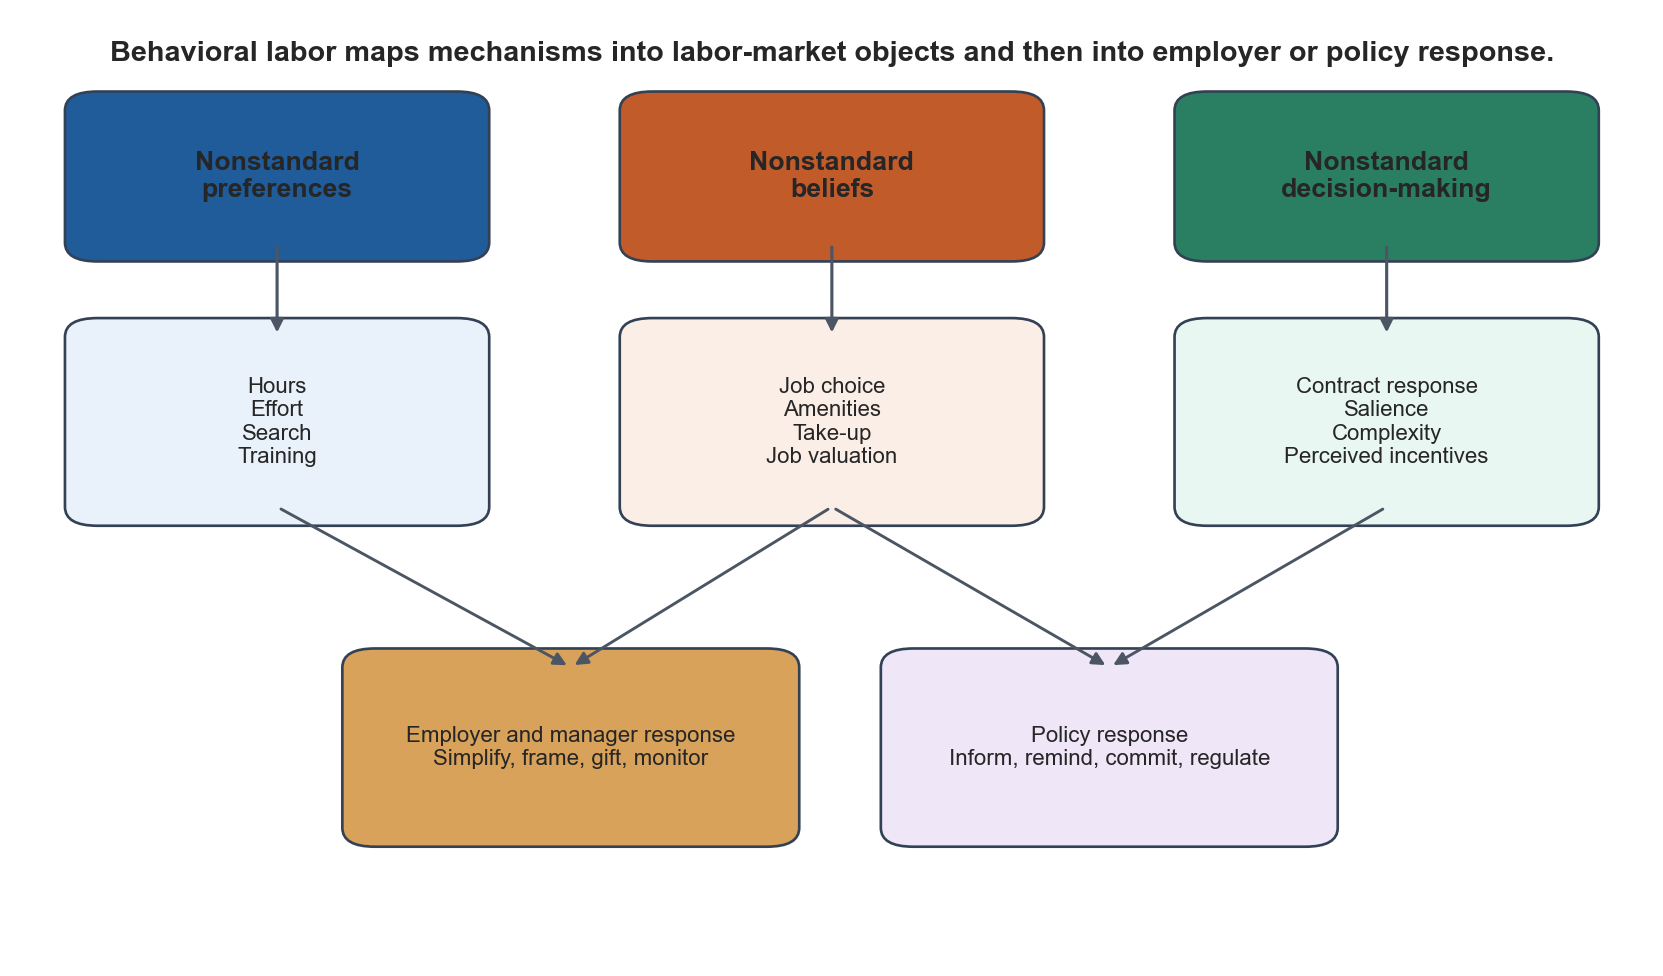
\includegraphics[height=0.72\textheight,keepaspectratio]{12-dellavigna-taxonomy-to-labor.png}
\end{center}
\end{frame}

\begin{frame}{Benchmark labor choice and the behavioral wedge}
\[
\max_{h \in \mathcal{H}} U(c,h)
\quad \text{s.t.} \quad
c = y + w h - T(w h + y)
\]

\[
a_i \in \arg\max_{a \in \mathcal{A}}
\left\{
\tilde{\mathbb{E}}_i[u_i(c(a),x(a))] - \tilde{\kappa}_i(a)
\right\}
\]

\begin{itemize}
    \item Preferences change what workers want.
    \item Beliefs change what workers think.
    \item Decision-making frictions change how true incentives become perceived incentives.
\end{itemize}
\end{frame}

\begin{frame}{Benchmark versus behavioral wedges}
\begin{center}
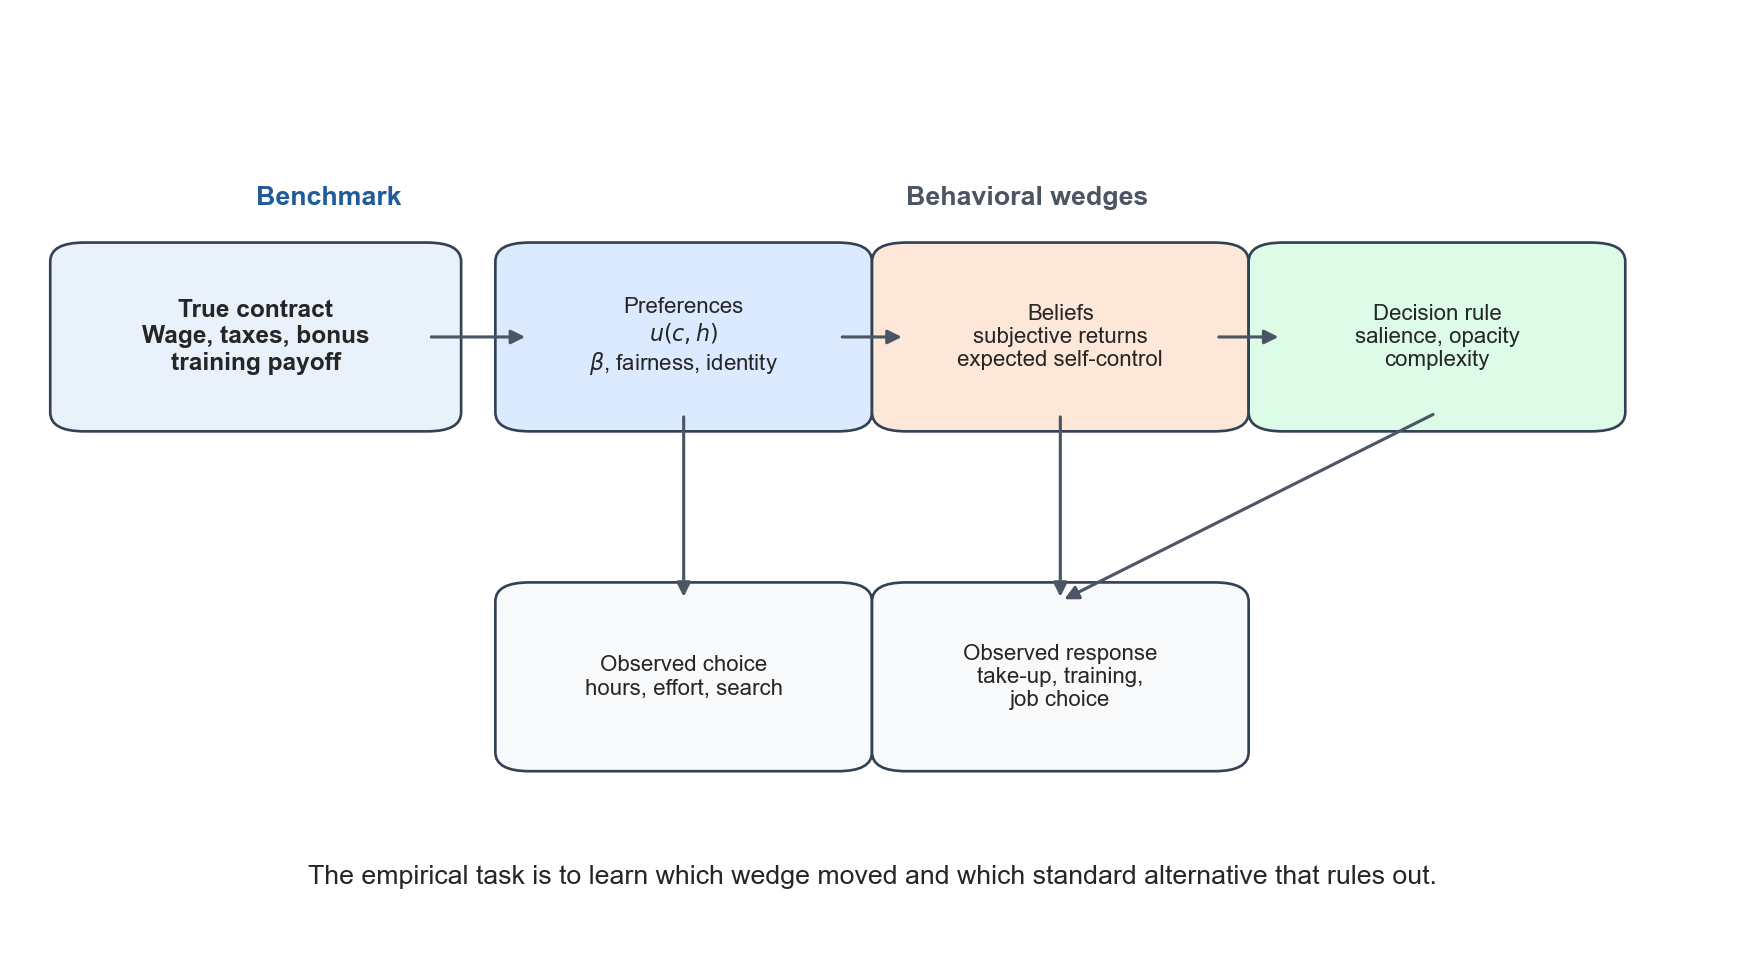
\includegraphics[height=0.72\textheight,keepaspectratio]{12-benchmark-vs-behavioral-wedges.png}
\end{center}
\end{frame}

\begin{frame}{Nonstandard preferences in labor}
\[
U_t = u(c_t,h_t) + \beta \sum_{s=t+1}^T \delta^{s-t} u(c_s,h_s)
\]

\[
u_i = w_i - \psi(e_i) + \alpha_i (w_i-r_i) + \rho_i G_i e_i
\]

\begin{itemize}
    \item Present bias matters for search, training, and habit formation.
    \item Fairness, reciprocity, and reference points matter for effort and contract response.
    \item The standard alternative to rule out is simple spot-market optimization with stable preferences.
\end{itemize}
\end{frame}

\begin{frame}{Nonstandard beliefs in labor}
\[
\tilde{R}_{it}
=
\mathbb{E}_{it}^{\,s}\!\left[w_{t+1}(k_{t+1}) - w_t(k_t)\right]
\]

\begin{itemize}
    \item Subjective beliefs shape search intensity, training take-up, and job valuation.
    \item Expectation errors are different from low objective returns.
    \item Measuring beliefs is often part of identification, not an optional add-on.
\end{itemize}
\end{frame}

\begin{frame}{Nonstandard decision-making in labor}
\[
\tilde{w} = \lambda w + (1-\lambda)\bar{w}
\]

\begin{itemize}
    \item Workers respond to perceived incentives, not always to true incentives.
    \item Complexity, salience, framing, and administrative burden can all attenuate response.
    \item Week 11 policy delivery and Week 12 behavioral labor meet here.
\end{itemize}
\end{frame}

\begin{frame}{Employers, managers, and policy respond too}
\begin{itemize}
    \item Firms can simplify, frame, gift, monitor, screen, or offer commitment.
    \item Some organizations exploit biases; others accommodate or offset them.
    \item Behavioral labor is partly about environment design, not only about worker mistakes.
\end{itemize}
\end{frame}

\begin{frame}{Empirical design toolkit}
\begin{center}
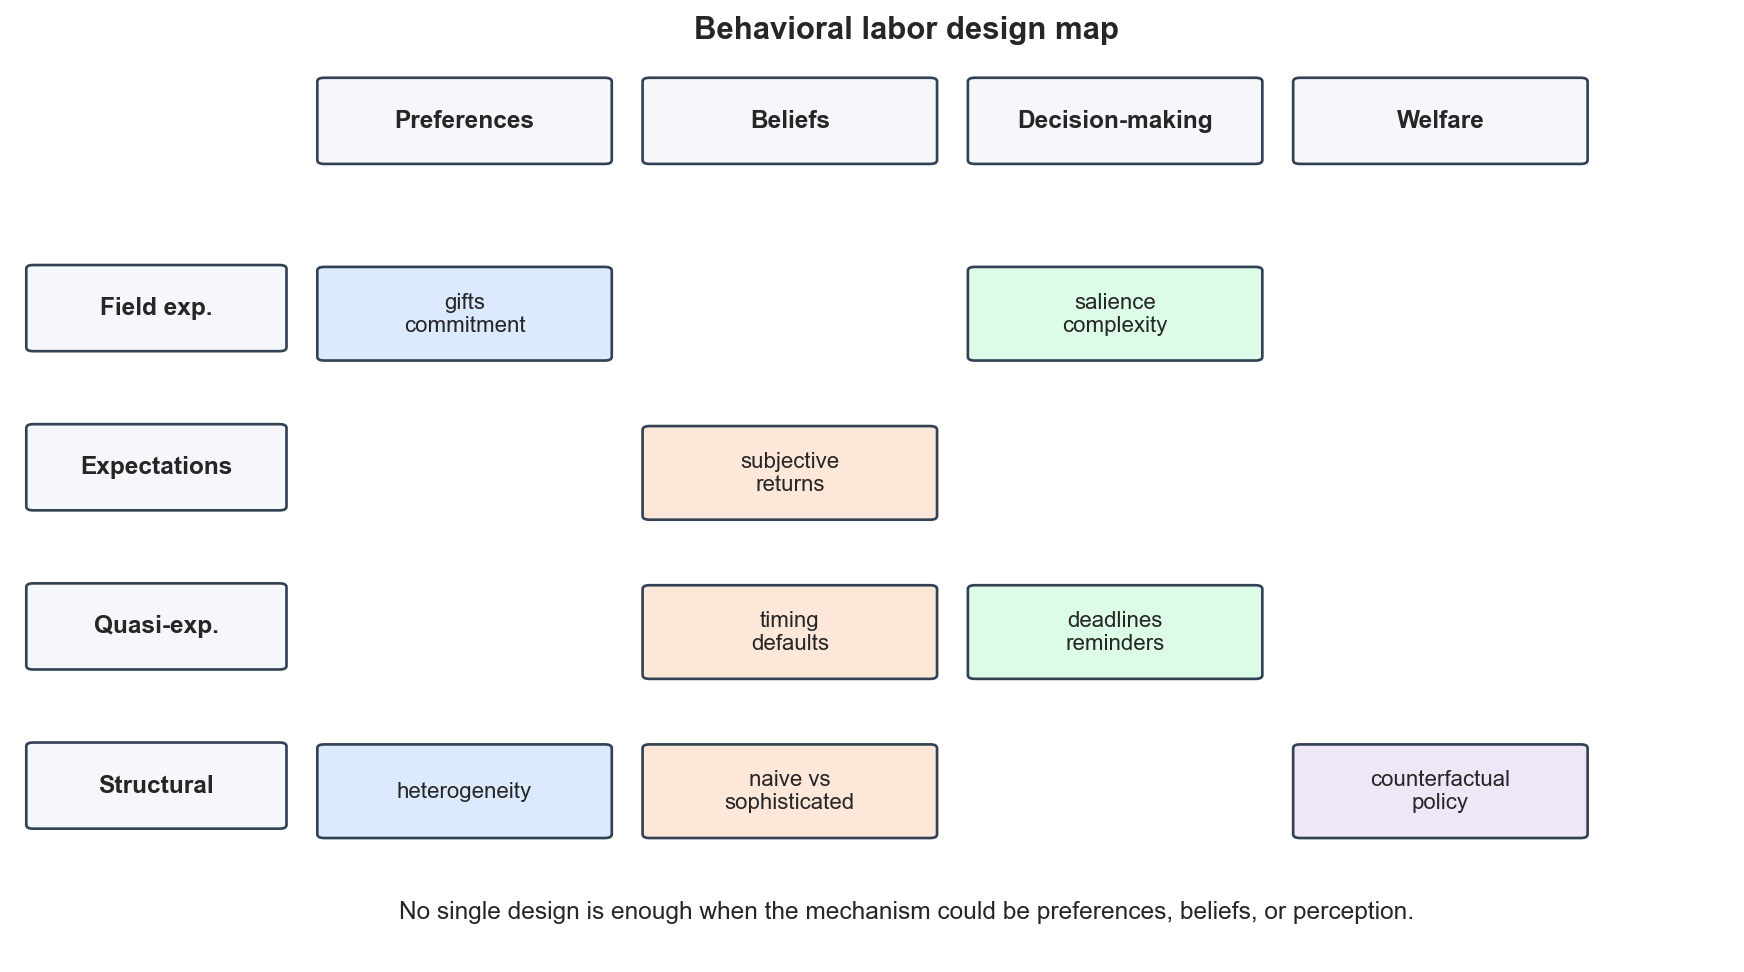
\includegraphics[height=0.72\textheight,keepaspectratio]{12-behavioral-labor-design-map.png}
\end{center}
\end{frame}

\begin{frame}{How identification works}
\begin{itemize}
    \item Field experiments isolate gifts, reminders, commitment, or complexity while holding the true contract fixed.
    \item Expectation-based designs measure subjective returns and perceived eligibility directly.
    \item Quasi-experiments are persuasive when timing, salience, or default rules move while statutory incentives do not.
    \item Structural estimation is most useful when the question is mechanism, counterfactual design, or welfare.
\end{itemize}
\end{frame}

\begin{frame}{Welfare and behavioral policy interpretation}
\[
W_i(a)=U_i^{LR}(a)-U_i^{LR}(a_i^{obs})
\]

\begin{itemize}
    \item Positive response is not the same as welfare improvement.
    \item Internalities, sophistication, learning, and the normative benchmark all matter.
    \item Behavioral labor requires a view on what choices should reveal.
\end{itemize}
\end{frame}

\begin{frame}{Market responses and welfare map}
\begin{center}
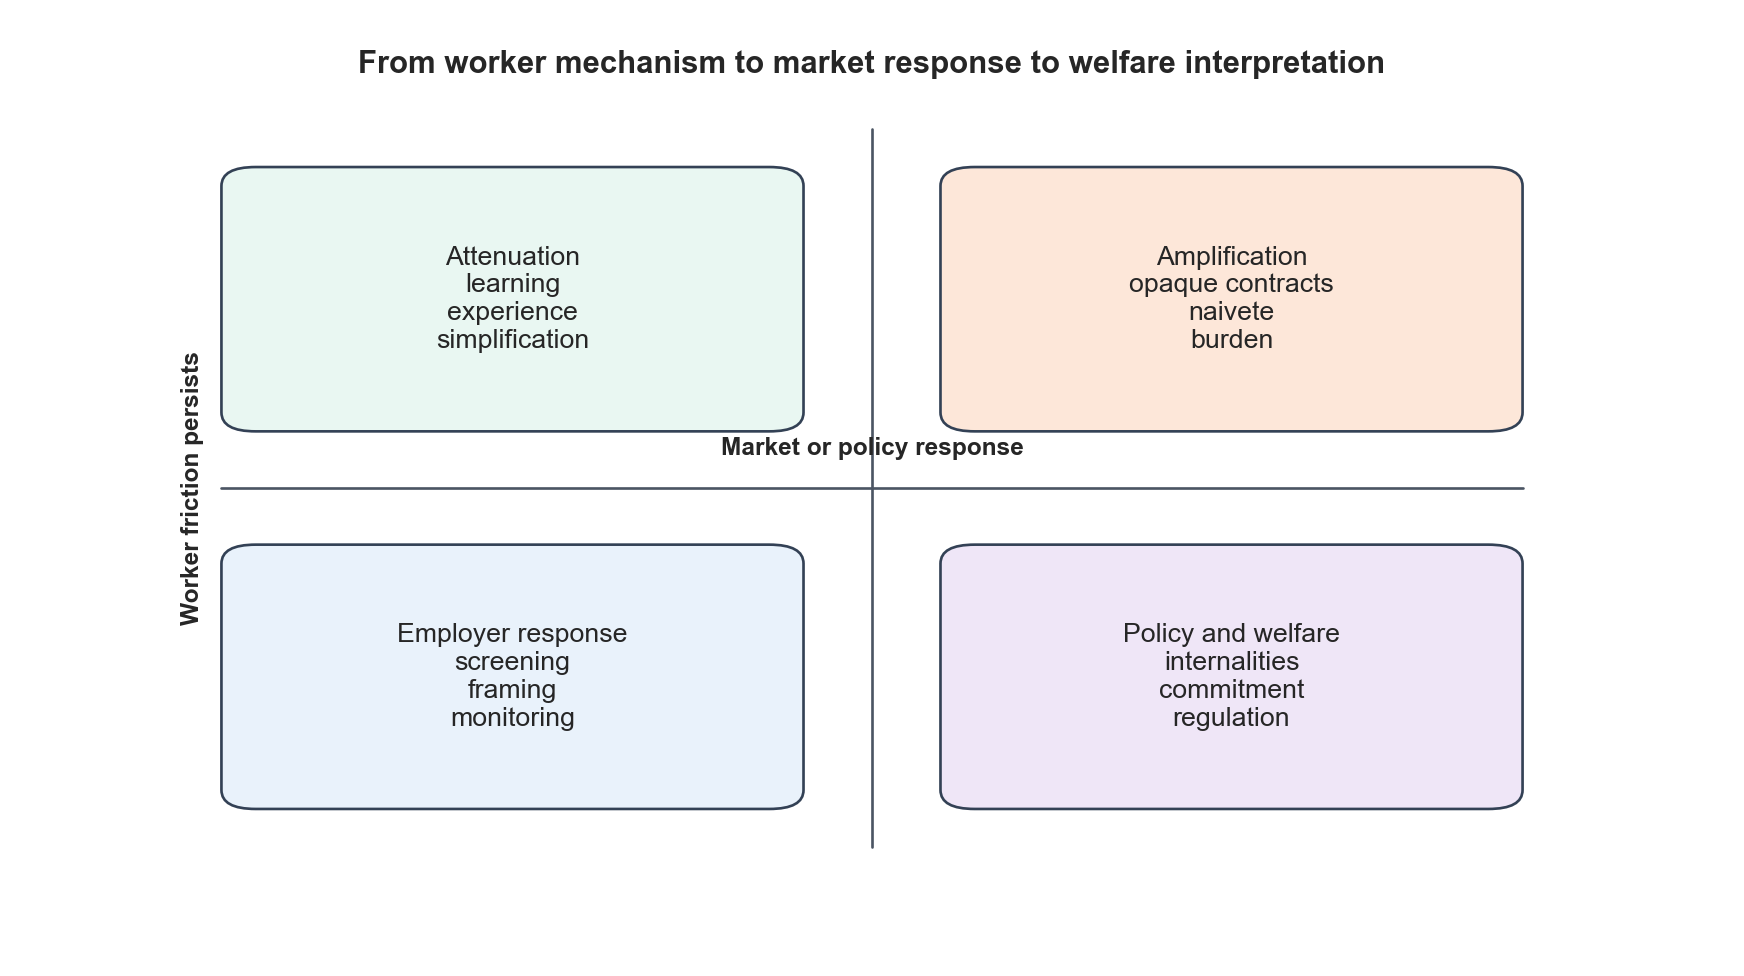
\includegraphics[height=0.72\textheight,keepaspectratio]{12-market-responses-and-welfare.png}
\end{center}
\end{frame}

\begin{frame}{Field map and bridge to a full course}
\begin{itemize}
    \item Self-control and dynamic labor supply.
    \item Fairness, reciprocity, and gift exchange at work.
    \item Identity, norms, and job choice.
    \item Attention, salience, and complexity.
    \item Beliefs, expectations, and perceived returns.
    \item Employer design and behavioral personnel economics.
    \item Welfare and behavioral policy design.
\end{itemize}
\end{frame}

\begin{frame}{Takeaways}
\begin{itemize}
    \item Behavioral labor is strongest when it produces distinctive predictions on labor-market margins.
    \item The benchmark matters: preference, belief, and decision-making wedges imply different tests.
    \item Employer and policy response are part of the field, not side notes.
    \item Week 12 closes Labor I by turning worker-side frictions into a field map.
\end{itemize}
\end{frame}

\appendix

\begin{frame}{Appendix: optional extension block}
\begin{itemize}
    \item Structural behavioral estimation and policy counterfactuals.
    \item Dynamic self-control in job search.
    \item Behavioral personnel economics and contract design.
\end{itemize}
\end{frame}

\end{document}
